\documentclass[a4paper,11pt]{article}
\usepackage[utf8]{inputenc}
\usepackage[ngerman]{babel}
\usepackage{geometry}
\usepackage{graphicx}
\usepackage{amsmath}
\usepackage{hyperref}
\usepackage{enumitem}

\geometry{a4paper, top=2cm, bottom=2cm, left=2cm, right=2cm}	

\usepackage{xcolor}
\definecolor{ohm_red}{RGB}{192,0,0}


\usepackage{fancyhdr}


\usepackage{titling}
\pretitle{\begin{flushleft}\LARGE}
\posttitle{\end{flushleft}}
\preauthor{\begin{flushleft}\large}
\postauthor{\end{flushleft}}

\setlength{\parindent}{0pt}



\pretitle{\begin{flushleft}\huge\textbf{\textcolor{ohm_red}}}
\posttitle{\end{flushleft}}

\pretitle{\begin{flushleft}\huge\textbf{\textcolor{ohm_red}}\rule{\linewidth}{0.4mm}\\}
\posttitle{\\\rule{\linewidth}{0.4mm}\end{flushleft}}
\title{\textcolor{ohm_red}{Erwerb komplexer Verhaltensmuster mittels Reinforcement Learning}}

\date{}


\usepackage{enumitem}
\setlist{nosep}

\pagestyle{fancy}
\renewcommand{\headrulewidth}{0pt}
\fancyhead[L]{
\includegraphics[height=2.0cm]{img/logo_autonohm.png}}
\fancyhead[R]{veröffentlicht am \today}


\usepackage{sidecap}

\sidecaptionvpos{figure}{c}


\begin{document}

\maketitle
\thispagestyle{fancy}

\vspace*{-3cm}
\begin{figure}[h!]
    \centering
    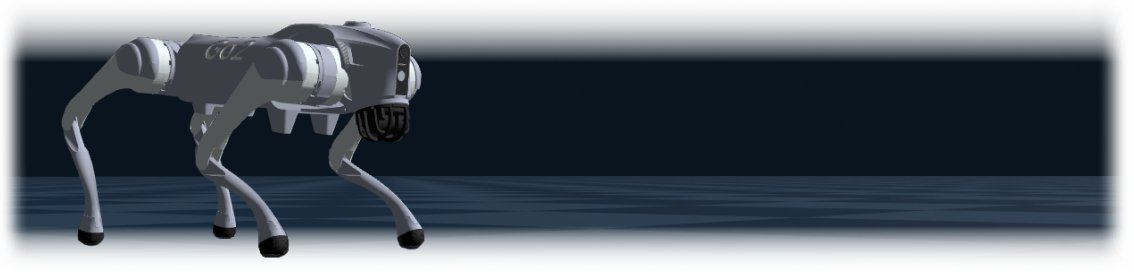
\includegraphics[height=4cm]{img/roboterhund.png}
    % \caption{Example Image}
    % \label{fig:example}
\end{figure}

Herkömmliche Verfahren der Regelungstechnik sind für die Regelung zwei- und vierbeiniger robotische Systeme aufgrund ihrer komplexen Kinematik nur bedingt geeignet.
Techniken des maschinellen Lernens wie beispielsweise das bestärkende Lernen (engl.: reinforcement learning) ermöglichen hingegen den gezielten Erwerb von Verhaltensmustern in simulierten Umgebungen und die darauffolgende Anwendung ebendieser in realen Umgebungen.\\\\
In dieser Arbeit sollen sinnvolle Verhaltensmuster für den Betrieb eines vierbeinigen Roboters identifiziert und erlernt werden. Der Fokus liegt dabei auf der Erstellung zielgerichteter Simulationsumgebungen, die mittels ausreichender Variabilität und Realitätsnähe die robuste Anwendung in realen Umgebungen begünstigen.
Für die Implementierung kann auf Open-Source-Software zurückgegriffen werden; ein vierbeiniger Roboter steht für Evaluationszwecke zur Verfügung.


\section*{Arbeitspakete}
\begin{itemize}[leftmargin=0.5cm]
    \item Recherche sinnvoller Verhaltensmuster
    \item Erstellung passender Simulationsumgebungen
    \item Training der gewünschten Verhaltensmuster mittels bestärkendem Lernen
    \item Test und Evaluation 
\end{itemize}

\section*{Voraussetzungen}
\begin{itemize}[leftmargin=0.5cm]
    \item Grundkenntnisse in Python
    \item Grundkenntnisse in 3D-Physiksimulation oder 3D-Modellierung (z.B. Isaac, Unity, Unreal, Blender)
    \item Grundkenntnisse im bestärkenden oder überwachten Lernen
\end{itemize}

\vspace{0.5cm}
Das Thema kann nach Abstimmung als Projekt-, Bachelor- oder Masterarbeit bearbeitet werden. 


\vfill
\textcolor{ohm_red}{\rule{\linewidth}{0.4mm}}
\textbf{\textcolor{ohm_red}{Labor für mobile Robotik}} \\
\begin{tabular}{@{}ll}
\textbf{Betreuer:} & Waldemar Haag \\
\textbf{E-Mail:}   & \href{mailto:waldemar.haag@th-nuernberg.de}{waldemar.haag@th-nuernberg.de} \\
\end{tabular}

\end{document}